\chapter{Konstrukce}

Základ mechanické konstukce tvoří extrudované hliníkové profily 30x30mm od firmy Missumi, konkrétně typ GFS6-3030. Profil má drážky které za pomocí zásuvných matek umožňují snadné přichycení dalšího příslušenství k profilu. Stejně tak spojování profilů je díky drážkám velice jednoduché. Vzhledem k tomu, že v celé konstrukci je zapotřebí velké množství spojů, vycházelo by použití originálních spojek draho. V nášledujiící tabulce je seznam riginálních dílů Misumi potřebných pro jeden spoj a  jejich cena.

\begin{table}[h!]
  \caption{Cena originálních dílů Misumi potřebných na jeden spoj (v Kč a včetně DPH). }
  \begin{center}
  	\small
	  \begin{tabular}{|c|c|c|c|}
	    \hline
	    	Název dílu	& Kód dílu	& Cena		&Počet ks	\\
	    \hline\hline

		Rohová spojka 	& HBLTS6	& 37		& 1		\\
		\hline
		Zásuvná matka 	& HNTP6-6 	& 16		& 2		\\
		\hline
	    \hline
	  \end{tabular}
  \end{center}
\end{table}


Jen spojky k sestavení rámu by tak přišly na přibližně 2000Kč. Proto byla zvolena úspornější varianta za použití 3D tisku FDM technologií. Díl HNTP6-6 byl nahrazen M6 matkou vsazenou do vytištěného dílu a rohová spojka HBLTS6 byla nahrazena celá tištěným dílem. Bez započtení energií a amortizace stroje vyšla cena plastových dílů na jeden spoj pod 5 Kč, což je výrazná úspora oproti 69Kč v originálních dílech.

Dle zadání má automat být schopen osazovat DPS o velikosti 150x250mm. Při návrhu velikosti pracovní plochy bylo také nutné počítat s prostorem pro zásobníky součástek a kameru. Jelikož bylo použito lineárního vedení s typyzovanou délkou po 10cm, zvolil jsem délku vedení pro osu X 60cm a pro osu Y 40cm. Při započtení rozměrů samotné osazovací hlavy tak šlo počítat s reálnou pracovní plochou přibližně 300x500 mm. Pro samotnou desku 150x250 mm a požadovaných 20 zásobnících na součástky je to dostatečně velký prostor.



\section{Řešení pojezdů pro osy X a Y}

Konstrukci pojezdů pro osy X a Y lze realizovat z běžně dostupných součástí třemi různými způsoby. Nejlevnější variantou je použití speciálně tvarovaných hliníkových profilů/kolejnic, po kterých budou jezdit ložiska nebo plastová kolečka. Použití ložisek v kombinaci s hliníkovou kolejnící není kvůli nízké tvrdosti hliníku příliš vhodné, časem pak dochází k vyježdění drázky v profilu. Proto se namísto ložiesk používají spíše tvrdé plasty jako je POM (Paraformaldehyd) konkrétně ve své variantě pod obchodním názvem Delrin. 

Ukázka hliníkového profilu MakerSlide s Delrinovými kolečky.

Delrinová kolečka jsou tvarována do tvaru písmene V stejně jako hliníková kolejnice. Tento systém zamezuje nežádoucímu pohybu osy ve směru kolmém na směr pohybu po kolejnici.

\section{Systém vodících tyčí}

Pojezd tvoří lineární ložiska jezdící po hlazené tyči. Hlazená tyč je buď uložená jen na koncích a ložisko ji celou obepíná, nebo je tyč po celé délce podepřená a lineární ložisko je s výřezem. Rozdíl mezi těmito variantamy je z hlediska maximální zatížitelnosti vedení. V našem případě by tak stačila varianta uložení  na koncích, váha celého pojezdu i s vakuovou pinzetou byla odhadována pod 1kg.

\section{Lineární vedení.}
Poslední zvažovanou a zároveň nejdražší možnosí bylo použití lineárního vedení. Tato varianta slibovala dosažení největších přesností. Dle zadání práce má být osazovací automat chopen osazovat součástky o velikosti 0805 pro které by bylo odatačující použití i první zmiňované varianty s Delrinovými kolečky. Osobním cílem ale bylo realizovat co nejpřesnější stroj který by byl schopen  osazovat i součástky o velikostech 0402. Proto bylo i přes svou vysokou cenu zvoleno právě toto řešení.

\section{Pohon os}
Pokud se omezíme na základní principy přenosu rotačního pohybu motoru na lineární pohyb, zůstávají dvě varianty jak osy pohánět. A to za pomocí řemenů a nebo šroubovicového systému.
Šroubovicový systém pracuje na podobném principu jako matka (pohyblivá část) našroubovaná na závitové tyči (šroubovice). Rozdílem je ale větší stoupání a jiný profil závitu minimalizující tření, což zvyšuje účinnost převodu. Takovým příkladem je trapézová štoubovice. Mnohem přesnější variantou je pak kuličková šroubovice. Místo závitu jsou v matce kuličky, které v ní recilkurují. Účinnos převodu je tak ješte vyšší než u trapézového šroubu. Při změně směru otáčení mají ale obě varianty tzv mrtvý chod. Tuto hysterezi je možné eliminovat použitím předepnutých matek matic.
Spojení šroubovice s motorem musí být přes pružnou spojku, aby se eliminovala chyba souososti.

Využití řemenů 
Řešení s řemeny je koncipováno tak, že přímo na hřídel motoru je přidělána řemenice. Druhá řemenice (nebo ložisko) je umístěna na opačném konci osy a mezi nimi je natažen uzavřený řemen.
Při správné volbě profilu řemenu je mrtvý chod zanedbatelný. Při velké délce řemenů může při jejich zatížení docházet k negativnímu propínání řemenů. Protot jsou řemeny vyztužovány tkaninou, nebo ocelovými dráty.

Použití řemenů výrazně zjednodušuje a zlevňuje celou konstrukci, proto byly do konstrukce zvoleny právě řemeny. Konkrétně řemen s profilem GT2, který je určen právě do aplikací s lineárním pohybem. Tvar zubu je zakulacený pro potlačení mrtvého chodu viz následující obrázek.


\section{Uspořádání os X a Y}

V předchozích kapitolách byly na základě úvah o přesnosti zařízení zvoleny pojezdy tvořené lineárním vedením poháněné řemeny. V této kapitole bude popsaná problematika uspořádání jednotlibých os.

Samotný polohovací systém osazovacího automatu pracuje v kartézském souřadnicovém systému.  Z konstrukčního hlediska bylo několik možností jak systém řešit. Základní konstrukční princip je, že každá osa má svůj vlastní motor (nebo více motorů), který ji pohání. Portálová konstrukce našeho osazovacího automatu by tak mohla vypadat dle následujícího obrázku.

\begin{figure}[h!]
  \centering
    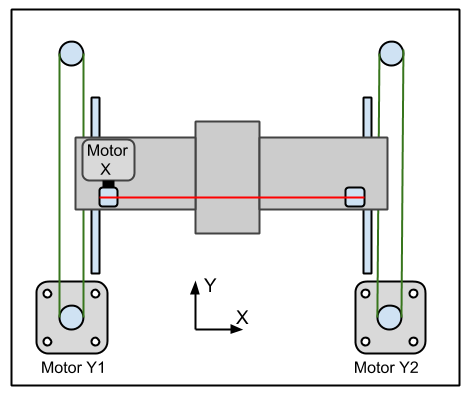
\includegraphics[width=0.6\linewidth]{obrazky/XY.png}%
    \caption{XY.}
    \label{fig:XY}
\end{figure}


V případě použití jendnoho motoru pro osu Y by bylo nutné spřažení pravé a levé části portálu, aby nedocházelo k nežádoucí rotaci při hnaní jen jedné části portálu. Alternativou by bylo na každou stranu portálu dát jeden motor a jejich otáčky řídit synchroně. 
Osa X by měla po boku vlastní motor a celá by byla uložená na ose Y. Tzn s pohybem v ose Y by se pohybovala i celá váha osy X. Na ose X je navíc ještě umístěna osa Z s vakuovou pipetou což je další hmota navíc. Dá se očekávat, že dynamické vlastnosti, rychlost a kompaktnost tohoto řešení nebude pro osazovací automat ideální (za předpokladu použití dostupných komponent).





\subsection{H-Bot}
Zajímavým uspořádáním, které úplně eliminuje nutnost aby se motor X pohyboval s osou Y z předchozího uspořádání je systém H-bot. V tomto řešení jsou motory staticky připevněné k rámu a řemen je uspořádán do tvaru H, proto H-bot. Hmota motorů se tak již nepohybuje s pohybem os, tudíž celá sestava bude mít menší setrvačnost a lze tak dosáhnout rychlých akcelerací a vysokých rychlostí. Systém využívá dva motory, kde pro pohyb mechanismu jen v jedné ose je zapotřebí obou motorů. Pokud se motory točí stejným směrem, pohybují s jednou osou. Pro pohyb v druhé ose se točí v protifázi.





\subsection{CoreXY}
Výše zmíněné nevýhoda systému H-bot jde eliminovat podobným, avšak mírně komplikovanějším uspořádáním zvaným coreXY. 

\begin{figure}[h!]
  \centering
    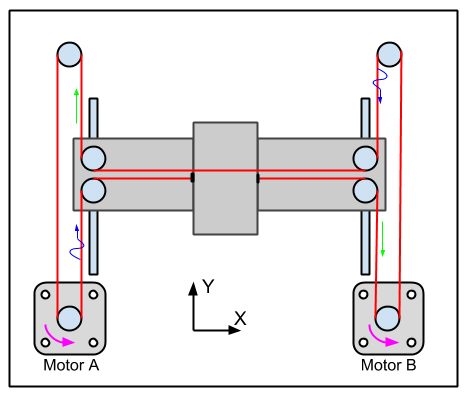
\includegraphics[width=0.6\linewidth]{obrazky/Hbot.png}%
    \caption{H-bot.}
    \label{fig:Hbot}
\end{figure}

Nevýhodou tohoto uspořádání je fakt, že síly působící na pohyblivý portál jsou v opačném směru což může vést k jeho mírné rotaci. Na obrázku je naznačen pohyb v pozitivním směru osy X, motor A i motor B se točí na stejnou stranu. Do obrázku byly naznačeny tahové a tlakové síly (zelená a modrá šipka), které by se měli v ideálním případě navzájem vyrušit. V reálném světě tomu tak není a portál má tendenci rotovat ve směru zelených šipek.
 S tímto systémem se tak dá dosahovat precizního polohování jen za předpokladu použití dostatečně tuhé konstrukce.





\subsection{CoreXY}
Výše zmíněné nevýhoda systému H-bot jde eliminovat podobným, avšak mírně komplikovanějším uspořádáním zvaným coreXY. 

\begin{figure}[h!]
  \centering
    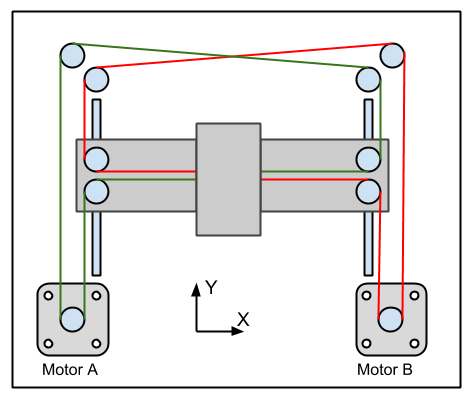
\includegraphics[width=0.6\linewidth]{obrazky/coreXY.png}%
    \caption{Core XY.}
    \label{fig:coreXY}
\end{figure}

Jak je vidět z obrázku, síly působící na portál působí oproti H bot již v jednom směru a nedochází tak k nechtěné rotaci portálu. 

